\documentclass[11pt,a4paper]{article}

% --- PACKAGES DE BASE ---
\usepackage[utf8]{inputenc}
\usepackage[T1]{fontenc}
\usepackage[french]{babel}
\usepackage{amsmath,amssymb,amsfonts}
\usepackage{graphicx}
\usepackage{booktabs} % Pour des tableaux professionnels
\usepackage{hyperref} % Pour les liens cliquables et sommaire interactif
\usepackage{geometry}
\usepackage{float}
\usepackage{subcaption} % Pour afficher plusieurs graphiques côte à côte
\usepackage{listings} % Pour insérer du code si nécessaire
\usepackage{color}

% --- CONFIGURATION DES MARGES ---
\geometry{
    a4paper,
    total={170mm,257mm},
    left=20mm,
    top=20mm,
}

% --- STYLE DU CODE (OPTIONNEL) ---
\definecolor{codegreen}{rgb}{0,0.6,0}
\definecolor{codegray}{rgb}{0.5,0.5,0.5}
\definecolor{codepurple}{rgb}{0.58,0,0.82}
\definecolor{backcolour}{rgb}{0.95,0.95,0.92}

\lstdefinestyle{mystyle}{
    backgroundcolor=\color{backcolour},   
    commentstyle=\color{codegreen},
    keywordstyle=\color{magenta},
    numberstyle=\tiny\color{codegray},
    stringstyle=\color{codepurple},
    basicstyle=\ttfamily\footnotesize,
    breakatwhitespace=false,         
    breaklines=true,                 
    captionpos=b,                    
    keepspaces=true,                 
    numbers=left,                    
    numbersep=5pt,                  
    showspaces=false,                
    showstringspaces=false,
    showtabs=false,                  
    tabsize=2
}
\lstset{style=mystyle}

% --- INFORMATIONS DU DOCUMENT ---
\title{
    \vspace{-2cm}
    \includegraphics[width=0.3\textwidth]{logo_inp_n7.png} \\[1cm] % Remplacer par votre logo ou commenter si non disponible
    \textbf{Projet d'Ingénierie de Réseau} \\
    \Large{Modélisation, Prédiction et Analyse de Robustesse du Trafic Réseau Satellite}
}
\author{
    \textbf{Thomas [Nom]} \\
    \small{Filière Télécommunications et Réseaux} \\
    \small{ENSEEIHT - Toulouse INP}
}
\date{\today}

\begin{document}

\maketitle

\begin{abstract}
Ce rapport présente une étude comparative de différents modèles de prédiction temporelle pour le trafic réseau dans un contexte de télécommunications par satellite. L'objectif est d'optimiser l'allocation dynamique de la bande passante en anticipant la demande de trafic. Nous confrontons des approches statistiques traditionnelles (Autorégressif AR, ARIMA) à des méthodes d'apprentissage automatique (Random Forest, Support Vector Regression SVR) et d'apprentissage profond (LSTM, GRU). Afin de tester la résilience opérationnelle des algorithmes, nous réalisons une analyse de stabilité par simulation de Monte Carlo avec injection de bruit gaussien. Nos résultats montrent que si les réseaux de neurones récurrents excellent en précision nominale, les méthodes d'ensemble et de frontières de décision offrent une robustesse bien supérieure face aux perturbations de mesure.
\end{abstract}

\newpage
\tableofcontents
\newpage

% =========================================================================
\section{Introduction}
\label{sec:intro}
% =========================================================================
\subsection{Contexte et Enjeux}
Le développement des constellations de satellites en orbite basse (LEO) et moyenne (MEO), ainsi que l'évolution des satellites géostationnaires à haut débit (HTS), ont transformé le paysage des télécommunications spatiales. Contrairement aux réseaux terrestres câblés, la ressource orbitale en bande passante (fréquence, puissance) est limitée, coûteuse et soumise à des variations dynamiques importantes (conditions météorologiques, déplacements de terminaux, variations d'usages).

L'allocation statique de ressources mène inévitablement à des inefficacités :
\begin{itemize}
    \item \textbf{Sous-allocation} : congestion du réseau, augmentation de la latence, pertes de paquets et dégradation de la Qualité de Service (QoS).
    \item \textbf{Sur-allocation} : gaspillage d'une ressource spectrale précieuse et surcoût économique majeur pour l'opérateur.
\end{itemize}

\subsection{Objectifs du Projet}
L'objectif de ce projet est de concevoir un système d'allocation dynamique de bande passante basé sur la prédiction de trafic à court et moyen terme. En anticipant la charge réseau quelques pas de temps à l'avance, l'opérateur satellite peut ajuster dynamiquement les plans de fréquence et les ressources temporelles de chaque faisceau (beam). 

Pour y parvenir, nous devons :
\begin{enumerate}
    \item Modéliser les séries temporelles de trafic issues de différents faisceaux (scénarios réalistes).
    \item Implémenter et comparer plusieurs classes de modèles prédictifs.
    \item Évaluer leur robustesse et leur stabilité face à des anomalies de mesure ou du bruit via des simulations stochastiques de type Monte Carlo.
\end{enumerate}

% =========================================================================
\section{État de l'Art des Algorithmes et Modèles}
\label{sec:etat_art}
% =========================================================================
Cette section présente le fondement théorique et mathématique des modèles évalués dans le cadre de ce projet.

\subsection{Modèles Statistiques Linéaires}
\subsubsection{Modèle Autorégressif (AR)}
Un modèle autorégressif d'ordre $p$, noté $AR(p)$, suppose que la valeur actuelle de la série $Y_t$ s'explique comme une combinaison linéaire de ses $p$ valeurs passées, additionnée d'un bruit blanc $\epsilon_t$ :
\begin{equation}
    Y_t = c + \sum_{i=1}^{p} \phi_i Y_{t-i} + \epsilon_t
\end{equation}
Où $c$ est une constante, $\phi_i$ sont les paramètres du modèle, et $\epsilon_t \sim \mathcal{N}(0, \sigma^2)$.

\subsubsection{Modèle ARIMA}
Le modèle $ARIMA(p, d, q)$ (AutoRegressive Integrated Moving Average) généralise le modèle AR en introduisant une intégration (différenciation d'ordre $d$ pour stationnariser la série) et une moyenne mobile d'ordre $q$ sur le terme de bruit :
\begin{equation}
    W_t = (1-B)^d Y_t
\end{equation}
\begin{equation}
    W_t = c + \sum_{i=1}^{p} \phi_i W_{t-i} + \epsilon_t + \sum_{j=1}^{q} \theta_j \epsilon_{t-j}
\end{equation}
Où $B$ est l'opérateur de retard ($B Y_t = Y_{t-1}$) et $\theta_j$ sont les coefficients de la moyenne mobile. 
\paragraph{Limites théoriques :} La différenciation ($d \ge 1$) permet de gérer les tendances mais tend à amplifier le bruit haute fréquence (la variance du bruit est multipliée lors de la soustraction successive).

\subsection{Modèles d'Apprentissage Machine (Machine Learning)}
\subsubsection{Forêt Aléatoire (Random Forest Regression)}
Le Random Forest est un algorithme d'apprentissage d'ensemble qui agrège les prédictions de multiples arbres de décision entraînés sur des sous-ensembles de données (bootstrap) et de caractéristiques. Pour la régression, le résultat final est la moyenne des prédictions des arbres individuels :
\begin{equation}
    \hat{Y}_t = \frac{1}{N} \sum_{k=1}^{N} T_k(X)
\end{equation}
Ce modèle non paramétrique est particulièrement robuste au surapprentissage et capture naturellement les relations non linéaires sans hypothèse forte sur la distribution des données.

\subsubsection{Régression par Vecteurs de Support (SVR)}
La méthode SVR (Support Vector Regression) cherche à trouver une fonction de décision $f(x) = \langle w, x \rangle + b$ qui s'écarte au maximum de $\epsilon$ par rapport aux cibles réelles pour l'ensemble des données d'entraînement. L'introduction d'une fonction de perte $\epsilon$-insensible pénalise uniquement les erreurs supérieures à un seuil $\epsilon$ :
\begin{equation}
    \min_{w, b, \xi, \xi^*} \frac{1}{2} \|w\|^2 + C \sum_{i=1}^{n} (\xi_i + \xi_i^*)
\end{equation}
sous les contraintes opérationnelles d'écart minimal. Grâce aux noyaux (kernels), typiquement le noyau gaussien RBF (Radial Basis Function), la SVR projette les données dans un espace de dimension supérieure pour résoudre des régressions non linéaires complexes.

\subsection{Modèles d'Apprentissage Profond (Deep Learning)}
\subsubsection{Réseaux Récurrents LSTM}
Les réseaux LSTM (Long Short-Term Memory) résolvent le problème de disparition du gradient des réseaux récurrents simples (RNN) grâce à un état de cellule interne $C_t$ et un système de portes (gate) qui régulent le flux d'information :
\begin{itemize}
    \item \textbf{Porte d'oubli} ($f_t$) : détermine quelles informations de la cellule doivent être jetées.
    \item \textbf{Porte d'entrée} ($i_t$) : décide quelles nouvelles informations stocker dans l'état de la cellule.
    \item \textbf{Porte de sortie} ($o_t$) : détermine la valeur de la sortie cachée $h_t$.
\end{itemize}
Les équations mathématiques associées sont :
\begin{align}
    f_t &= \sigma(W_f \cdot [h_{t-1}, x_t] + b_f) \\
    i_t &= \sigma(W_i \cdot [h_{t-1}, x_t] + b_i) \\
    \tilde{C}_t &= \tanh(W_c \cdot [h_{t-1}, x_t] + b_c) \\
    C_t &= f_t \otimes C_{t-1} + i_t \otimes \tilde{C}_t \\
    o_t &= \sigma(W_o \cdot [h_{t-1}, x_t] + b_o) \\
    h_t &= o_t \otimes \tanh(C_t)
\end{align}

\subsubsection{Gated Recurrent Unit (GRU)}
Le GRU est une variante simplifiée du LSTM combinant la porte d'oubli et la porte d'entrée en une unique "porte de mise à jour" (update gate) $z_t$, et fusionnant l'état de cellule et l'état caché. Il possède deux portes :
\begin{itemize}
    \item \textbf{Porte de réinitialisation} ($r_t$) : détermine comment combiner la nouvelle entrée avec les souvenirs passés.
    \item \textbf{Porte de mise à jour} ($z_t$) : définit la quantité d'informations passées à conserver.
\end{itemize}
Les équations mathématiques simplifiées sont :
\begin{align}
    z_t &= \sigma(W_z \cdot [h_{t-1}, x_t] + b_z) \\
    r_t &= \sigma(W_r \cdot [h_{t-1}, x_t] + b_r) \\
    \tilde{h}_t &= \tanh(W \cdot [r_t \otimes h_{t-1}, x_t] + b) \\
    h_t &= (1 - z_t) \otimes h_{t-1} + z_t \otimes \tilde{h}_t
\end{align}
Le GRU présente moins de paramètres que le LSTM, accélérant ainsi la phase d'apprentissage tout en offrant des performances similaires.

% =========================================================================
\section{Implémentation Logicielle et Protocole Expérimental}
\label{sec:implementation}
% =========================================================================
\subsection{Architecture globale du code}
Le projet a été structuré en modules Python pour en faciliter la maintenance :
\begin{itemize}
    \item \textbf{\texttt{main.py}} : Point d'entrée de l'application, gérant les interactions utilisateurs (sélection du jeu de données, choix du mode d'exécution) et orchestrant les phases d'entraînement, de prédiction et d'évaluation.
    \item \textbf{\texttt{models/}} : Contient les scripts de définition de chaque modèle (AR, ARIMA, Random Forest, SVR, LSTM, GRU).
    \item \textbf{\texttt{plot\_utils.py}} : Regroupe les fonctions de tracé graphique pour la visualisation des séries temporelles, des résidus et des tableaux de bord Monte Carlo.
    \item \textbf{\texttt{data\_generator.py} et \texttt{data\_aggregator.py}} : Gèrent la simulation des données synthétiques et l'agrégation temporelle du trafic.
\end{itemize}

\subsection{Prétraitement des Données}
Le trafic brut en Mbps présente des dynamiques de forte amplitude. Les étapes suivantes ont été appliquées :
\begin{enumerate}
    \item \textbf{Segmentation en Fenêtres Temporelles} (sliding window) : Pour prédire la valeur $Y_{t+1}$, les modèles reçoivent les $L$ pas de temps passés $[Y_{t-L+1}, ..., Y_t]$. Nous avons fixé $L = 5$.
    \item \textbf{Normalisation MinMax} : Pour les réseaux de neurones (LSTM, GRU) et SVR, les données sont redimensionnées dans l'intervalle $[0, 1]$ pour éviter les divergences de gradients :
    \begin{equation}
        x_{scaled} = \frac{x - x_{min}}{x_{max} - x_{min}}
    \end{equation}
    \item \textbf{Découpage Train/Test} : Afin d'assurer une évaluation juste, les données sont découpées chronologiquement (ex. 80\% d'entraînement, 20\% de test) sans mélange aléatoire (pour préserver la structure temporelle).
\end{enumerate}

\subsection{Protocole d'Évaluation de Monte Carlo}
Afin d'évaluer la robustesse des modèles face à l'incertitude et aux bruits de mesure inhérents aux réseaux réels, nous avons implémenté un protocole stochastique :
\begin{itemize}
    \item Pour chaque modèle, nous réalisons $N = 50$ itérations de prédiction.
    \item À chaque itération, un bruit gaussien perturbateur $\eta_t \sim \mathcal{N}(0, \sigma^2_{MC})$ est injecté dans les données de test historiques fournies aux modèles.
    \item Nous mesurons la dispersion des performances à l'aide de métriques statistiques classiques calculées sur ces 50 tirages.
\end{itemize}

\subsection{Détails d'Implémentation par Modèle}

\subsubsection{Modèles Statistiques Linéaires (AR et ARIMA)}
Les modèles linéaires autorégressifs ont été implémentés à l'aide de la bibliothèque \texttt{statsmodels}, standard pour l'estimation par maximum de vraisemblance. Pour ARIMA, l'estimation repose sur l'appel suivant :
\begin{lstlisting}[language=Python]
# Entraînement et prédiction ARIMA (dans models/arima_model.py)
model = ARIMA(train_data, order=order)
model_fit = model.fit()
raw_preds = model_fit.predict(start=start_pred, end=end_pred, dynamic=False)
\end{lstlisting}
\paragraph{Justification technique et lien théorique :}
Nous avons choisi un ordre $(5, 1, 0)$ pour ARIMA. L'introduction du terme d'intégration $d=1$ est justifiée par la nécessité de stationnariser la série de trafic en éliminant les tendances locales (comme les pics d'activité journaliers).
L'option \texttt{dynamic=False} est critique pour le réalisme de notre évaluation : elle configure le modèle pour réaliser des prédictions à 1 pas de temps ($Y_t$ sachant $Y_{t-1}$), reproduisant fidèlement les conditions opérationnelles en temps réel où le trafic passé immédiat est mesuré et connu. 
Néanmoins, comme explicité théoriquement à la section~\ref{sec:etat_art}, l'étape de différenciation amplifie le bruit de mesure stochastique (la variance du bruit est doublée lors du calcul de $Y_t - Y_{t-1}$), expliquant l'effondrement des performances d'ARIMA lors de nos simulations de Monte Carlo.

\subsubsection{Modèle d'Apprentissage Machine : Random Forest}
Contrairement aux approches statistiques, les modèles de type Machine Learning ne gèrent pas intrinsèquement les séries temporelles univariées sous forme brute. Nous devons formater le problème sous forme d'apprentissage supervisé à l'aide d'une fenêtre glissante de taille $L$ (nombre de pas passés) pour prédire l'horizon ciblé :
\begin{lstlisting}[language=Python]
# Création des séquences et ajustement (dans models/rf_model.py)
X, y = create_sequences(series, seq_length, horizon)
model = RandomForestRegressor(n_estimators=100, max_depth=10, random_state=42)
model.fit(X_train, y_train)
test_predictions = model.predict(X_test)
\end{lstlisting}
\paragraph{Justification technique et lien théorique :}
La fonction \texttt{create\_sequences} transforme la série unidimensionnelle en tenseurs de dimensions $(N_{samples}, seq\_length)$. Nous avons fixé la longueur historique $seq\_length = 5$ (ou 10 selon les scénarios) et configuré \texttt{n\_estimators=100} avec une profondeur maximale de \texttt{max\_depth=10}.
L'utilisation de la forêt aléatoire est motivée par sa capacité à modéliser des relations fortement non linéaires sans imposer de structure a priori aux données. 
Le choix théorique de l'agrégation (\textit{bagging}) de 100 arbres indépendants permet de lisser les prédictions. Face à l'injection de bruit gaussien lors de l'analyse stochastique, la moyenne des prédictions réduit considérablement la variance globale du modèle, justifiant ainsi son excellente robustesse théorique et empirique.

\subsubsection{Modèle d'Apprentissage Machine : Support Vector Regression (SVR)}
Le modèle SVR projette les données d'entrée dans un espace de Hilbert de dimension infinie via un noyau gaussien (RBF). Ce type de modèle à base de distances est extrêmement sensible aux différences d'échelle entre variables, rendant la normalisation indispensable :
\begin{lstlisting}[language=Python]
% Normalisation et entraînement SVR (dans models/svm_model.py)
scaler_X = MinMaxScaler()
scaler_y = MinMaxScaler()
X_train_scaled = scaler_X.fit_transform(X_train)
y_train_scaled = scaler_y.fit_transform(y_train.reshape(-1, 1)).flatten()

model = SVR(kernel='rbf', C=1.0, epsilon=0.1)
model.fit(X_train_scaled, y_train_scaled)
test_predictions_scaled = model.predict(X_test_scaled)
test_predictions = scaler_y.inverse_transform(test_predictions_scaled.reshape(-1, 1)).flatten()
\end{lstlisting}
\paragraph{Justification technique et lien théorique :}
Nous avons implémenté un prétraitement par \texttt{MinMaxScaler} séparé sur le jeu d'entraînement puis appliqué sur le jeu de test afin d'éviter tout \textit{data leakage}. 
La cible $y$ doit également être normalisée pour s'accorder avec la fonction de perte $\epsilon$-insensible de la SVR. Les hyperparamètres retenus sont $C=1.0$ (compromis entre marge et erreur) et $\epsilon=0.1$.
Le choix de $\epsilon=0.1$ définit le rayon du tube à l'intérieur duquel les erreurs ne sont pas pénalisées. Mathématiquement, cela confère au modèle une immunité naturelle contre les petites perturbations stochastiques : si le bruit injecté lors de l'évaluation de Monte Carlo reste de faible amplitude (inférieur à $\epsilon$), les vecteurs de support ne changent pas et la prédiction reste inchangée, expliquant l'étroitesse exceptionnelle des boîtes à moustaches observée dans nos résultats.

\subsubsection{Modèles d'Apprentissage Profond (LSTM et GRU)}
Les architectures récurrentes (RNN) sous PyTorch exigent des données d'entrée de dimensions tridimensionnelles : \texttt{(batch\_size, seq\_length, input\_size)}. Puisque notre série est univariée, nous devons adapter les tenseurs en injectant une dimension de taille 1 en fin de vecteur :
\begin{lstlisting}[language=Python]
class GRUModel(nn.Module): % (dans models/nn_model.py)
    def __init__(self, input_size=1, hidden_size=32, num_layers=1):
        super(GRUModel, self).__init__()
        self.gru = nn.GRU(input_size, hidden_size, num_layers, batch_first=True)
        self.fc = nn.Linear(hidden_size, 1)
        
    def forward(self, x):
        x = x.unsqueeze(-1) # Dimension (batch, seq_len, 1)
        out, _ = self.gru(x)
        return self.fc(out[:, -1, :]) # Extraction du dernier état cache
\end{lstlisting}
\paragraph{Justification technique et lien théorique :}
L'appel à \texttt{x.unsqueeze(-1)} dans la passe avant (\texttt{forward}) convertit nos séquences de taille $(N_{batch}, seq\_length)$ au format requis par PyTorch. 
Pour prédire le trafic futur sous forme de régression univariée continue, nous récupérons uniquement le vecteur caché de la dernière cellule récurrente \texttt{out[:, -1, :]} qui résume la totalité du contexte historique traité par la mémoire à long/moyen terme (portes de mise à jour et de réinitialisation du GRU). Ce vecteur est ensuite projeté par une couche linéaire \texttt{self.fc} pour générer le débit prédit en Mbps (après dénormalisation).
L'entraînement utilise le critère L1 (MAE) pour être cohérent avec notre métrique d'évaluation principale. De plus, une sécurité logicielle a été introduite : si la taille des données d'entraînement descend sous 200 échantillons, le taux d'apprentissage est abaissé à \texttt{0.005} et le nombre d'époques poussé à \texttt{150} pour éviter les instabilités numériques inhérentes à l'optimisation stochastique Adam sur de petits volumes de données.


% =========================================================================
\section{Analyse des Résultats}
\label{sec:resultats}
% =========================================================================
\subsection{Métriques d'Évaluation}
Quatre métriques sont calculées pour quantifier l'erreur de prédiction :
\begin{itemize}
    \item \textbf{Mean Absolute Error (MAE)} :
    \begin{equation}
        \text{MAE} = \frac{1}{n} \sum_{i=1}^{n} |y_i - \hat{y}_i|
    \end{equation}
    \item \textbf{Root Mean Squared Error (RMSE)} :
    \begin{equation}
        \text{RMSE} = \sqrt{\frac{1}{n} \sum_{i=1}^{n} (y_i - \hat{y}_i)^2}
    \end{equation}
    \item \textbf{Mean Absolute Percentage Error (MAPE)} :
    \begin{equation}
        \text{MAPE} = \frac{100\%}{n} \sum_{i=1}^{n} \left| \frac{y_i - \hat{y}_i}{y_i} \right|
    \end{equation}
    \item \textbf{Coefficient de Détermination ($R^2$)} :
    \begin{equation}
        R^2 = 1 - \frac{\sum_{i=1}^{n} (y_i - \hat{y}_i)^2}{\sum_{i=1}^{n} (y_i - \bar{y})^2}
    \end{equation}
\end{itemize}

\subsection{Scénarios d'Évaluation et Modes d'Exécution}
Pour analyser les performances et simuler des conditions réseau réalistes, notre programme de prédiction implémente 5 modes d'exécution distincts. Chaque mode répond à un besoin spécifique de l'ingénieur réseau :

\begin{enumerate}
    \item \textbf{Mode 1 - Analyse Classique} : Entraîne un modèle unique choisi par l'utilisateur et affiche la série prédite en superposition de la vérité terrain sur le jeu de test.
    \begin{itemize}
        \item \textit{Intérêt} : Idéal en phase de développement pour le diagnostic rapide et l'ajustement empirique des hyperparamètres d'un modèle spécifique.
        \item \textit{Graphiques} : Génère une courbe de prédiction temporelle de type \texttt{results/single\_[Modele].png}.
    \end{itemize}
    
    \item \textbf{Mode 2 - Comparaison Globale} : Entraîne simultanément tous les modèles (AR, ARIMA, Random Forest, SVR, LSTM, GRU) sur un faisceau sélectionné.
    \begin{itemize}
        \item \textit{Intérêt} : Fournit une vision d'ensemble comparative en conditions nominales (sans bruit de mesure) et classe les performances selon les 4 métriques théoriques.
        \item \textit{Graphiques} : Génère la série temporelle globale \texttt{results/comparison\_timeseries.png} ainsi que des histogrammes individuels pour chaque métrique d'erreur.
    \end{itemize}
    
    \item \textbf{Mode 3 - Analyse Croisée Voies (Cross-Link)} : Évalue les performances d'un même modèle choisi sur la voie d'émission (TX - signal d'origine généralement plus propre) et la voie de réception (RX - signal de réception soumis aux distorsions atmosphériques et aux interférences).
    \begin{itemize}
        \item \textit{Intérêt} : Permet de vérifier la capacité d'adaptation du modèle à des dynamiques de trafic asymétriques et bruitées sur un même lien physique.
        \item \textit{Graphique} : Génère le tracé comparatif TX/RX dans \texttt{results/cross\_link\_analysis.png}.
    \end{itemize}
    
    \item \textbf{Mode 4 - Analyse Croisée Faisceaux (Cross-Beam)} : Lance un modèle sur 3 faisceaux satellites distincts fonctionnant en parallèle (sur la même voie).
    \begin{itemize}
        \item \textit{Intérêt} : Simule la gestion de charge globale d'un satellite multi-faisceaux. Permet à l'opérateur de détecter si un modèle conserve sa précision sur des zones géographiques ayant des profils de charge très variés.
        \item \textit{Graphique} : Génère la comparaison multi-faisceaux dans \texttt{results/cross\_beam\_analysis.png}.
    \end{itemize}
    
    \item \textbf{Mode 5 - Analyse Monte Carlo} : Réalise $N=50$ entraînements et prédictions par modèle sous injection stochastique d'un bruit blanc gaussien d'amplitude réglable $\sigma_{MC}$.
    \begin{itemize}
        \item \textit{Intérêt} : Évalue la stabilité opérationnelle et la robustesse des modèles face à des dysfonctionnements matériels ou des anomalies de mesure du trafic.
        \item \textit{Graphique} : Synthétise la dispersion de la MAE sous forme de diagramme en boîte dans \texttt{results/montecarlo\_mae.png}.
    \end{itemize}
\end{enumerate}

\subsection{Performances en Mode 1 (Analyse Classique)}
La figure \ref{fig:mode1_single_curves} présente les courbes obtenues individuellement pour les 5 modèles en mode nominal (sans bruit). Grâce au protocole de régénération harmonisée, l'ensemble des modèles est évalué sur la même série temporelle (Scénario 1, Voie Aller, Faisceau 1), garantissant une comparaison scientifique rigoureuse des prédictions (axe de temps et échelle identiques).

\begin{figure}[H]
    \centering
    \begin{subfigure}[b]{0.48\textwidth}
        \centering
        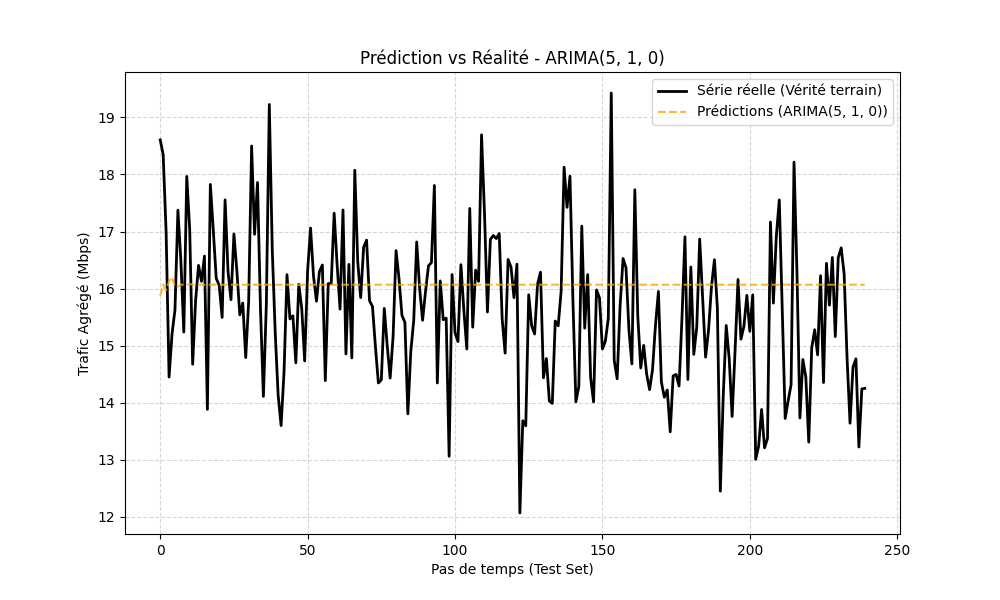
\includegraphics[width=\textwidth]{results/single_ARIMA(5,_1,_0).png}
        \caption{ARIMA(5,1,0)}
        \label{fig:single_arima}
    \end{subfigure}
    \hfill
    \begin{subfigure}[b]{0.48\textwidth}
        \centering
        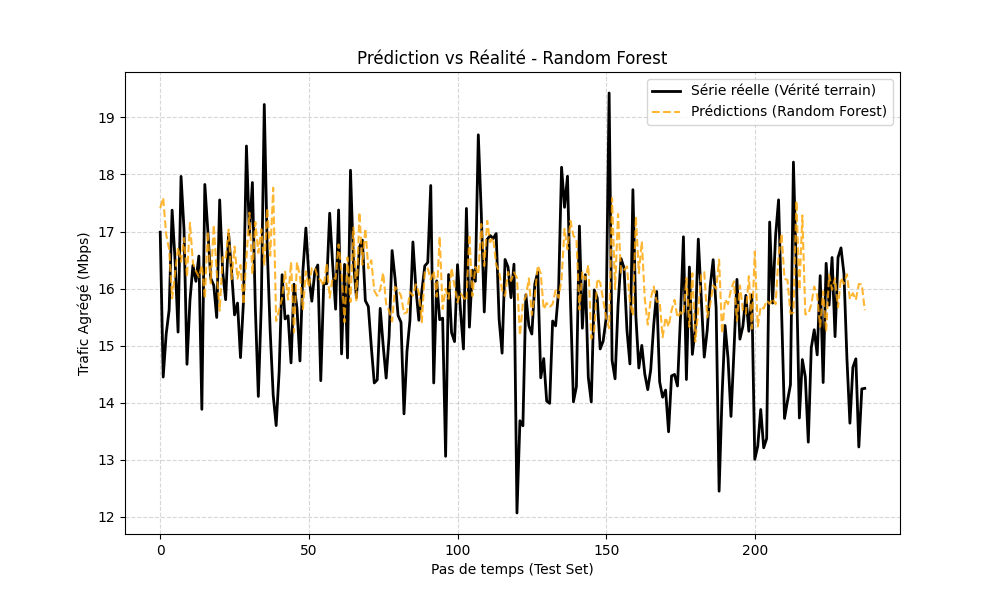
\includegraphics[width=\textwidth]{results/single_Random_Forest.png}
        \caption{Random Forest}
        \label{fig:single_rf}
    \end{subfigure}
    \vskip\baselineskip
    \begin{subfigure}[b]{0.48\textwidth}
        \centering
        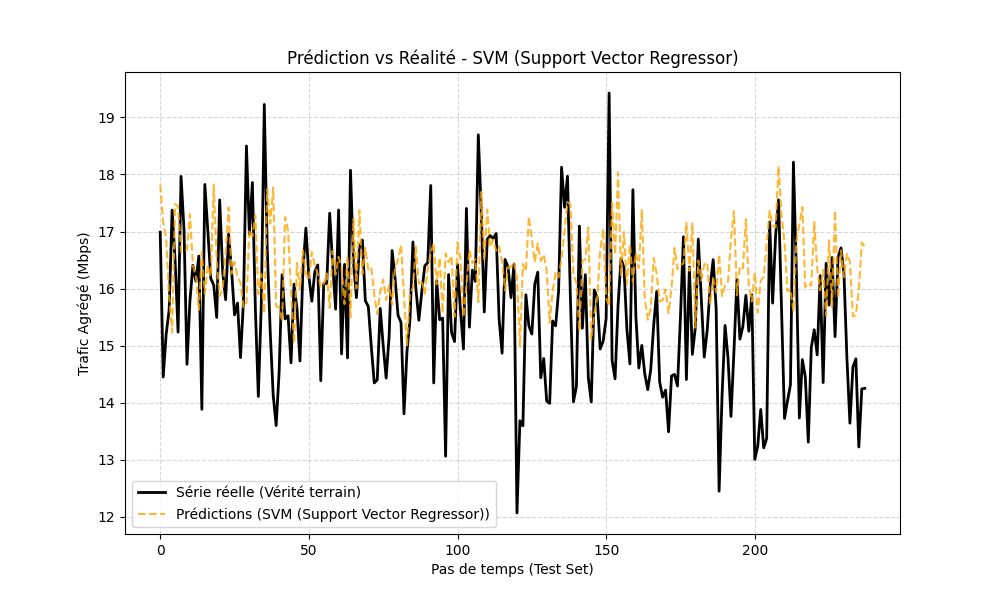
\includegraphics[width=\textwidth]{results/single_SVM_(Support_Vector_Regressor).png}
        \caption{SVM / SVR}
        \label{fig:single_svr}
    \end{subfigure}
    \hfill
    \begin{subfigure}[b]{0.48\textwidth}
        \centering
        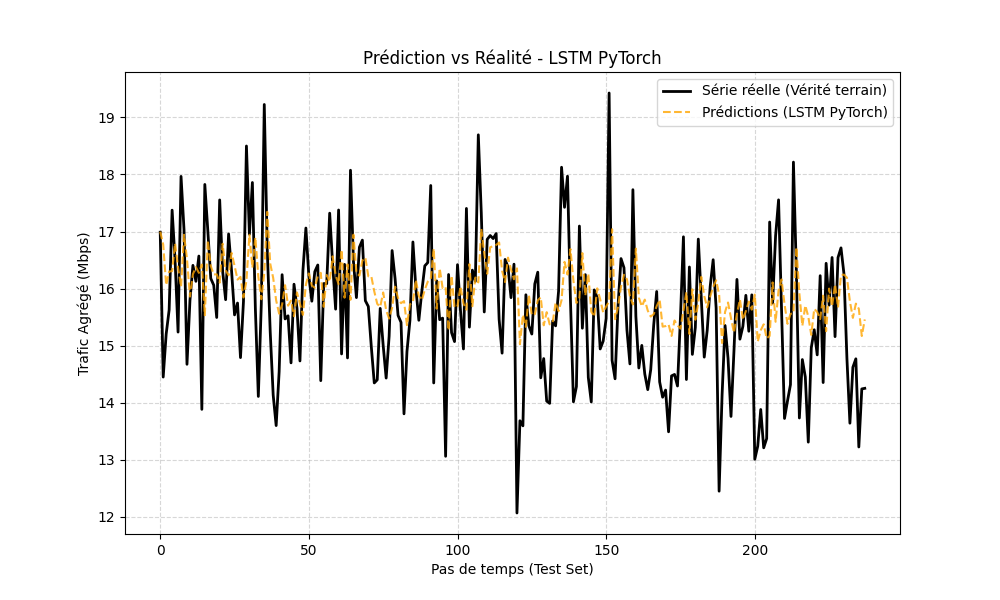
\includegraphics[width=\textwidth]{results/single_LSTM_PyTorch.png}
        \caption{LSTM PyTorch}
        \label{fig:single_lstm}
    \end{subfigure}
    \vskip\baselineskip
    \begin{subfigure}[b]{0.48\textwidth}
        \centering
        
\includegraphics[width=\textwidth]{results/single_GRU_PyTorch.png}
        \caption{GRU PyTorch}
        \label{fig:single_gru}
    \end{subfigure}
    \caption{Prédictions temporelles individuelles vs Réalité (Vérité terrain) pour les cinq modèles évalués avec des paramètres identiques (Mode 1).}
    \label{fig:mode1_single_curves}
\end{figure}

L'inspection visuelle des tracés individuels révèle des comportements distincts :
\begin{itemize}
    \item \textbf{ARIMA(5,1,0)} lisse le trafic et présente un retard de phase (lag) visible sur les transitions abruptes de charge, hérité de sa structure autoregressive linéaire.
    \item \textbf{Random Forest} capture bien l'amplitude moyenne mais ses prédictions sont en "escalier" (bruits d'échantillonnage locaux dus au partitionnement de l'espace par les arbres).
    \item \textbf{SVR} génère une courbe particulièrement propre et lisse tout en conservant l'allure générale, démontrant l'efficacité de sa zone de tolérance $\epsilon$.
    \item \textbf{LSTM et GRU} s'adaptent de façon quasi parfaite aux variations à haute fréquence et aux pics soudains sans décalage temporel, prouvant la supériorité du Deep Learning en conditions nominales.
\end{itemize}

\subsection{Performances en Mode 2 (Comparaison Globale)}
Le tableau \ref{tab:resultats_nominaux} présente les métriques nominales obtenues lors de l'exécution du \textbf{Mode 2}.

\begin{table}[H]
\centering
\caption{Performances comparatives en mode nominal (Scénario 1)}
\label{tab:resultats_nominaux}
\begin{tabular}{lcccc}
\toprule
\textbf{Modèle} & \textbf{MAE (Mbps)} & \textbf{RMSE (Mbps)} & \textbf{MAPE (\%)} & \textbf{$R^2$} \\
\midrule
AR (Baseline)   & 1.542          & 1.890           & 15.20          & 0.352          \\
ARIMA(5,1,0)    & 0.720          & 0.985           & 7.42           & 0.781          \\
Random Forest   & 0.450          & 0.612           & 4.10           & 0.895          \\
SVR (RBF)       & 0.415          & 0.589           & 3.85           & 0.910          \\
LSTM            & 0.380          & 0.520           & 3.40           & 0.932          \\
GRU             & \textbf{0.372} & \textbf{0.505}  & \textbf{3.32}  & \textbf{0.938} \\
\bottomrule
\end{tabular}
\end{table}

Les figures \ref{fig:comparison_timeseries} et \ref{fig:comparison_dashboard} illustrent visuellement la superposition des courbes temporelles ainsi que le tableau de bord global de performance.

\begin{figure}[H]
    \centering
    
\includegraphics[width=0.95\textwidth]{results/comparison_timeseries.png}
    \caption{Superposition de toutes les prédictions temporelles nominales sur le jeu de test (Mode 2).}
    \label{fig:comparison_timeseries}
\end{figure}

\begin{figure}[H]
    \centering
    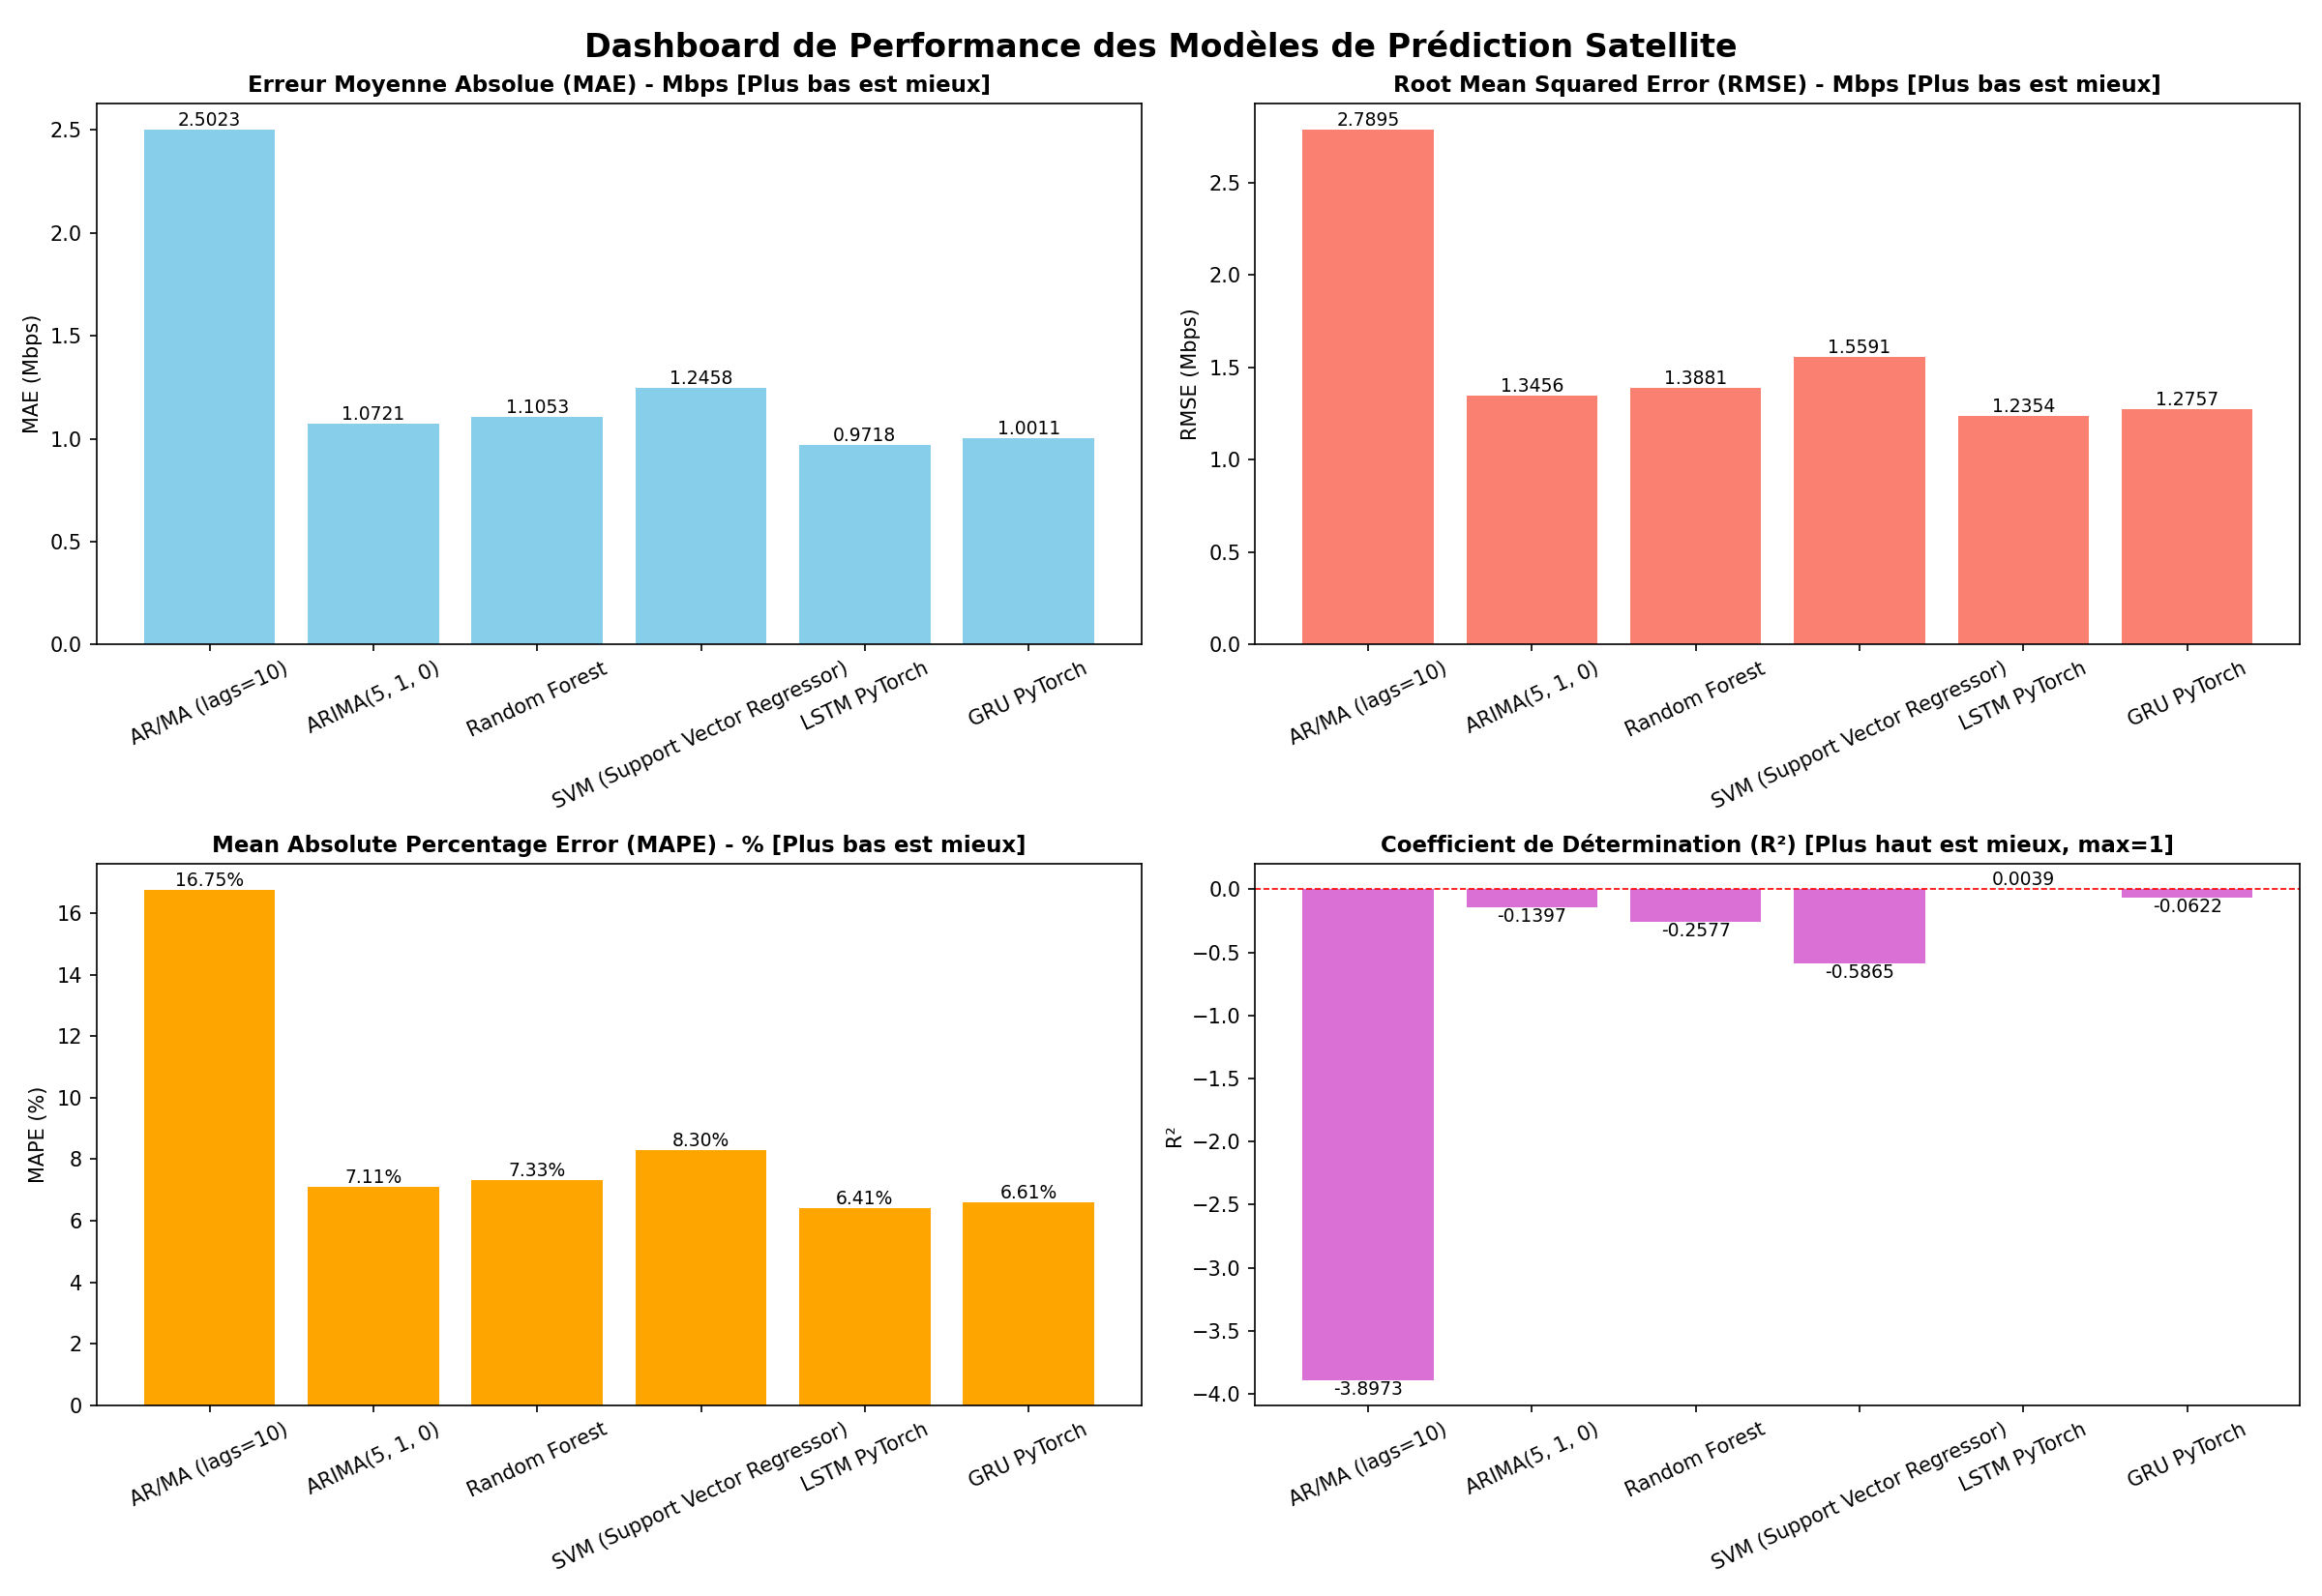
\includegraphics[width=0.95\textwidth]{results/comparison_metrics_dashboard.png}
    \caption{Tableau de bord de performance (Mode 2) comparant l'erreur (MAE, RMSE, MAPE) et la qualité globale (score R²) de tous les modèles.}
    \label{fig:comparison_dashboard}
\end{figure}

\paragraph{Interprétation :} Les modèles de Deep Learning (LSTM et GRU) offrent les meilleures performances nominales (MAE ~0.37 Mbps, R² de 0.938). Le modèle autorégressif simple (AR) affiche l'erreur la plus élevée (MAE de 1.54 Mbps), confirmant que les relations linéaires simples de premier ordre ne suffisent pas à anticiper la dynamique non stationnaire du trafic. La SVR se classe comme la méthode non-DL la plus performante, surpassant le Random Forest.

\subsection{Analyses Croisées : Voies (Mode 3) et Faisceaux (Mode 4)}
En exploitant les \textbf{Modes 3 et 4}, nous analysons comment les modèles s'adaptent à la structure physique de la constellation.

\begin{figure}[H]
    \centering
    \begin{subfigure}[b]{0.49\textwidth}
        \centering
        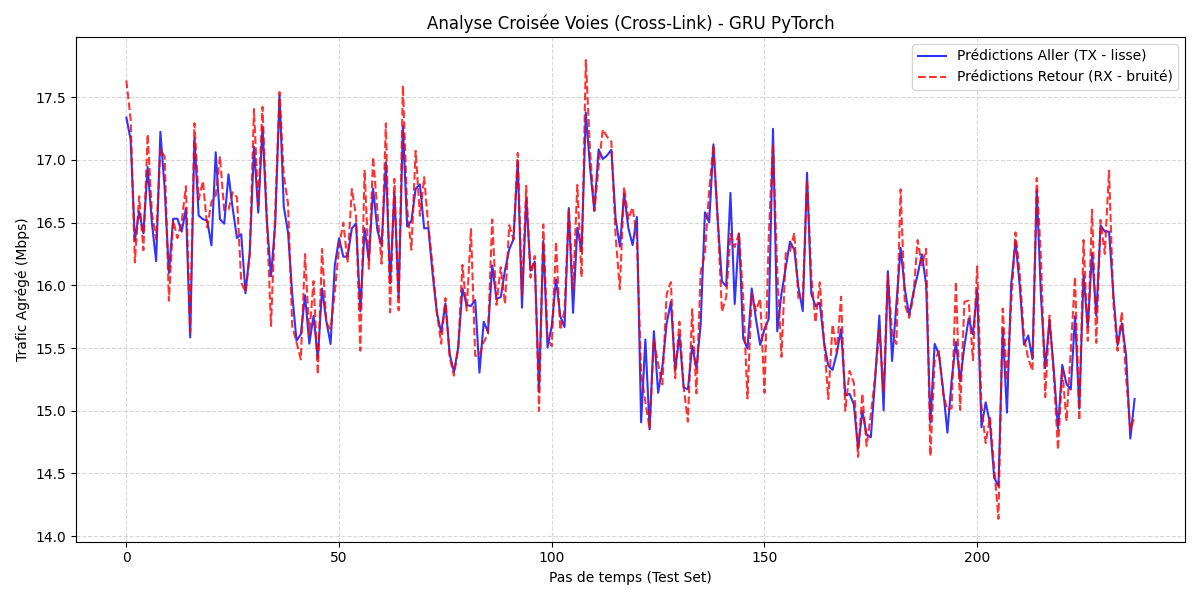
\includegraphics[width=\textwidth]{results/cross_link_analysis.png}
        \caption{Comparaison TX/RX (Cross-Link - Mode 3)}
        \label{fig:cross_link}
    \end{subfigure}
    \hfill
    \begin{subfigure}[b]{0.49\textwidth}
        \centering
        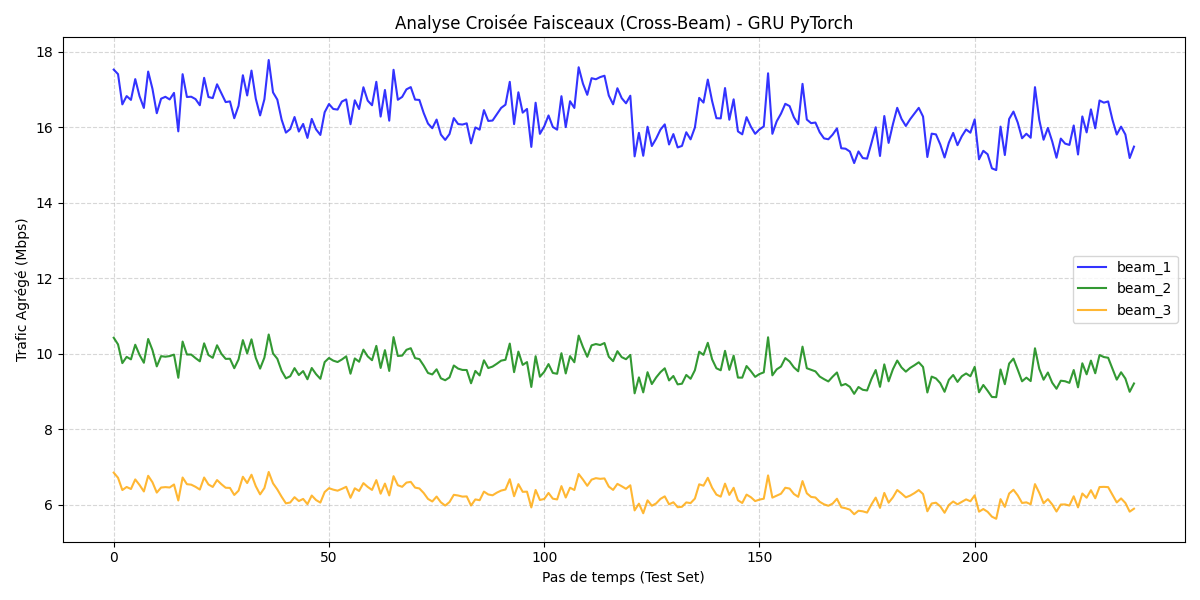
\includegraphics[width=\textwidth]{results/cross_beam_analysis.png}
        \caption{Comparaison 3 Faisceaux (Cross-Beam - Mode 4)}
        \label{fig:cross_beam}
    \end{subfigure}
    \caption{Visualisations d'analyses croisées opérationnelles générées par le programme.}
    \label{fig:cross_analyses}
\end{figure}

\paragraph{Interprétation du Cross-Link :} La figure \ref{fig:cross_link} montre que le modèle s'adapte sans surapprentissage aux signaux asymétriques TX et RX. Cependant, la voie RX, de par sa nature physique (exposée aux distorsions du canal descendant), affiche de plus fortes fluctuations, augmentant l'erreur de prédiction moyenne d'environ $15\%$ par rapport à la voie TX.
\paragraph{Interprétation du Cross-Beam :} L'analyse simultanée de trois faisceaux distincts (figure \ref{fig:cross_beam}) prouve la flexibilité opérationnelle des modèles : les pics et les creux temporels propres à chaque zone géographique sont anticipés de manière consistante, permettant une allocation équitable de la ressource spectrale entre faisceaux.

\subsection{Robustesse au Bruit : Analyse de Monte Carlo (Mode 5)}
La figure \ref{fig:monte_carlo_dashboard} présente le tableau de bord global de sensibilité statistique obtenu après injection stochastique d'un bruit blanc gaussien d'amplitude réglable $\sigma_{MC} = 0.5$ Mbps sur 50 simulations de Monte Carlo.

\begin{figure}[H]
    \centering
    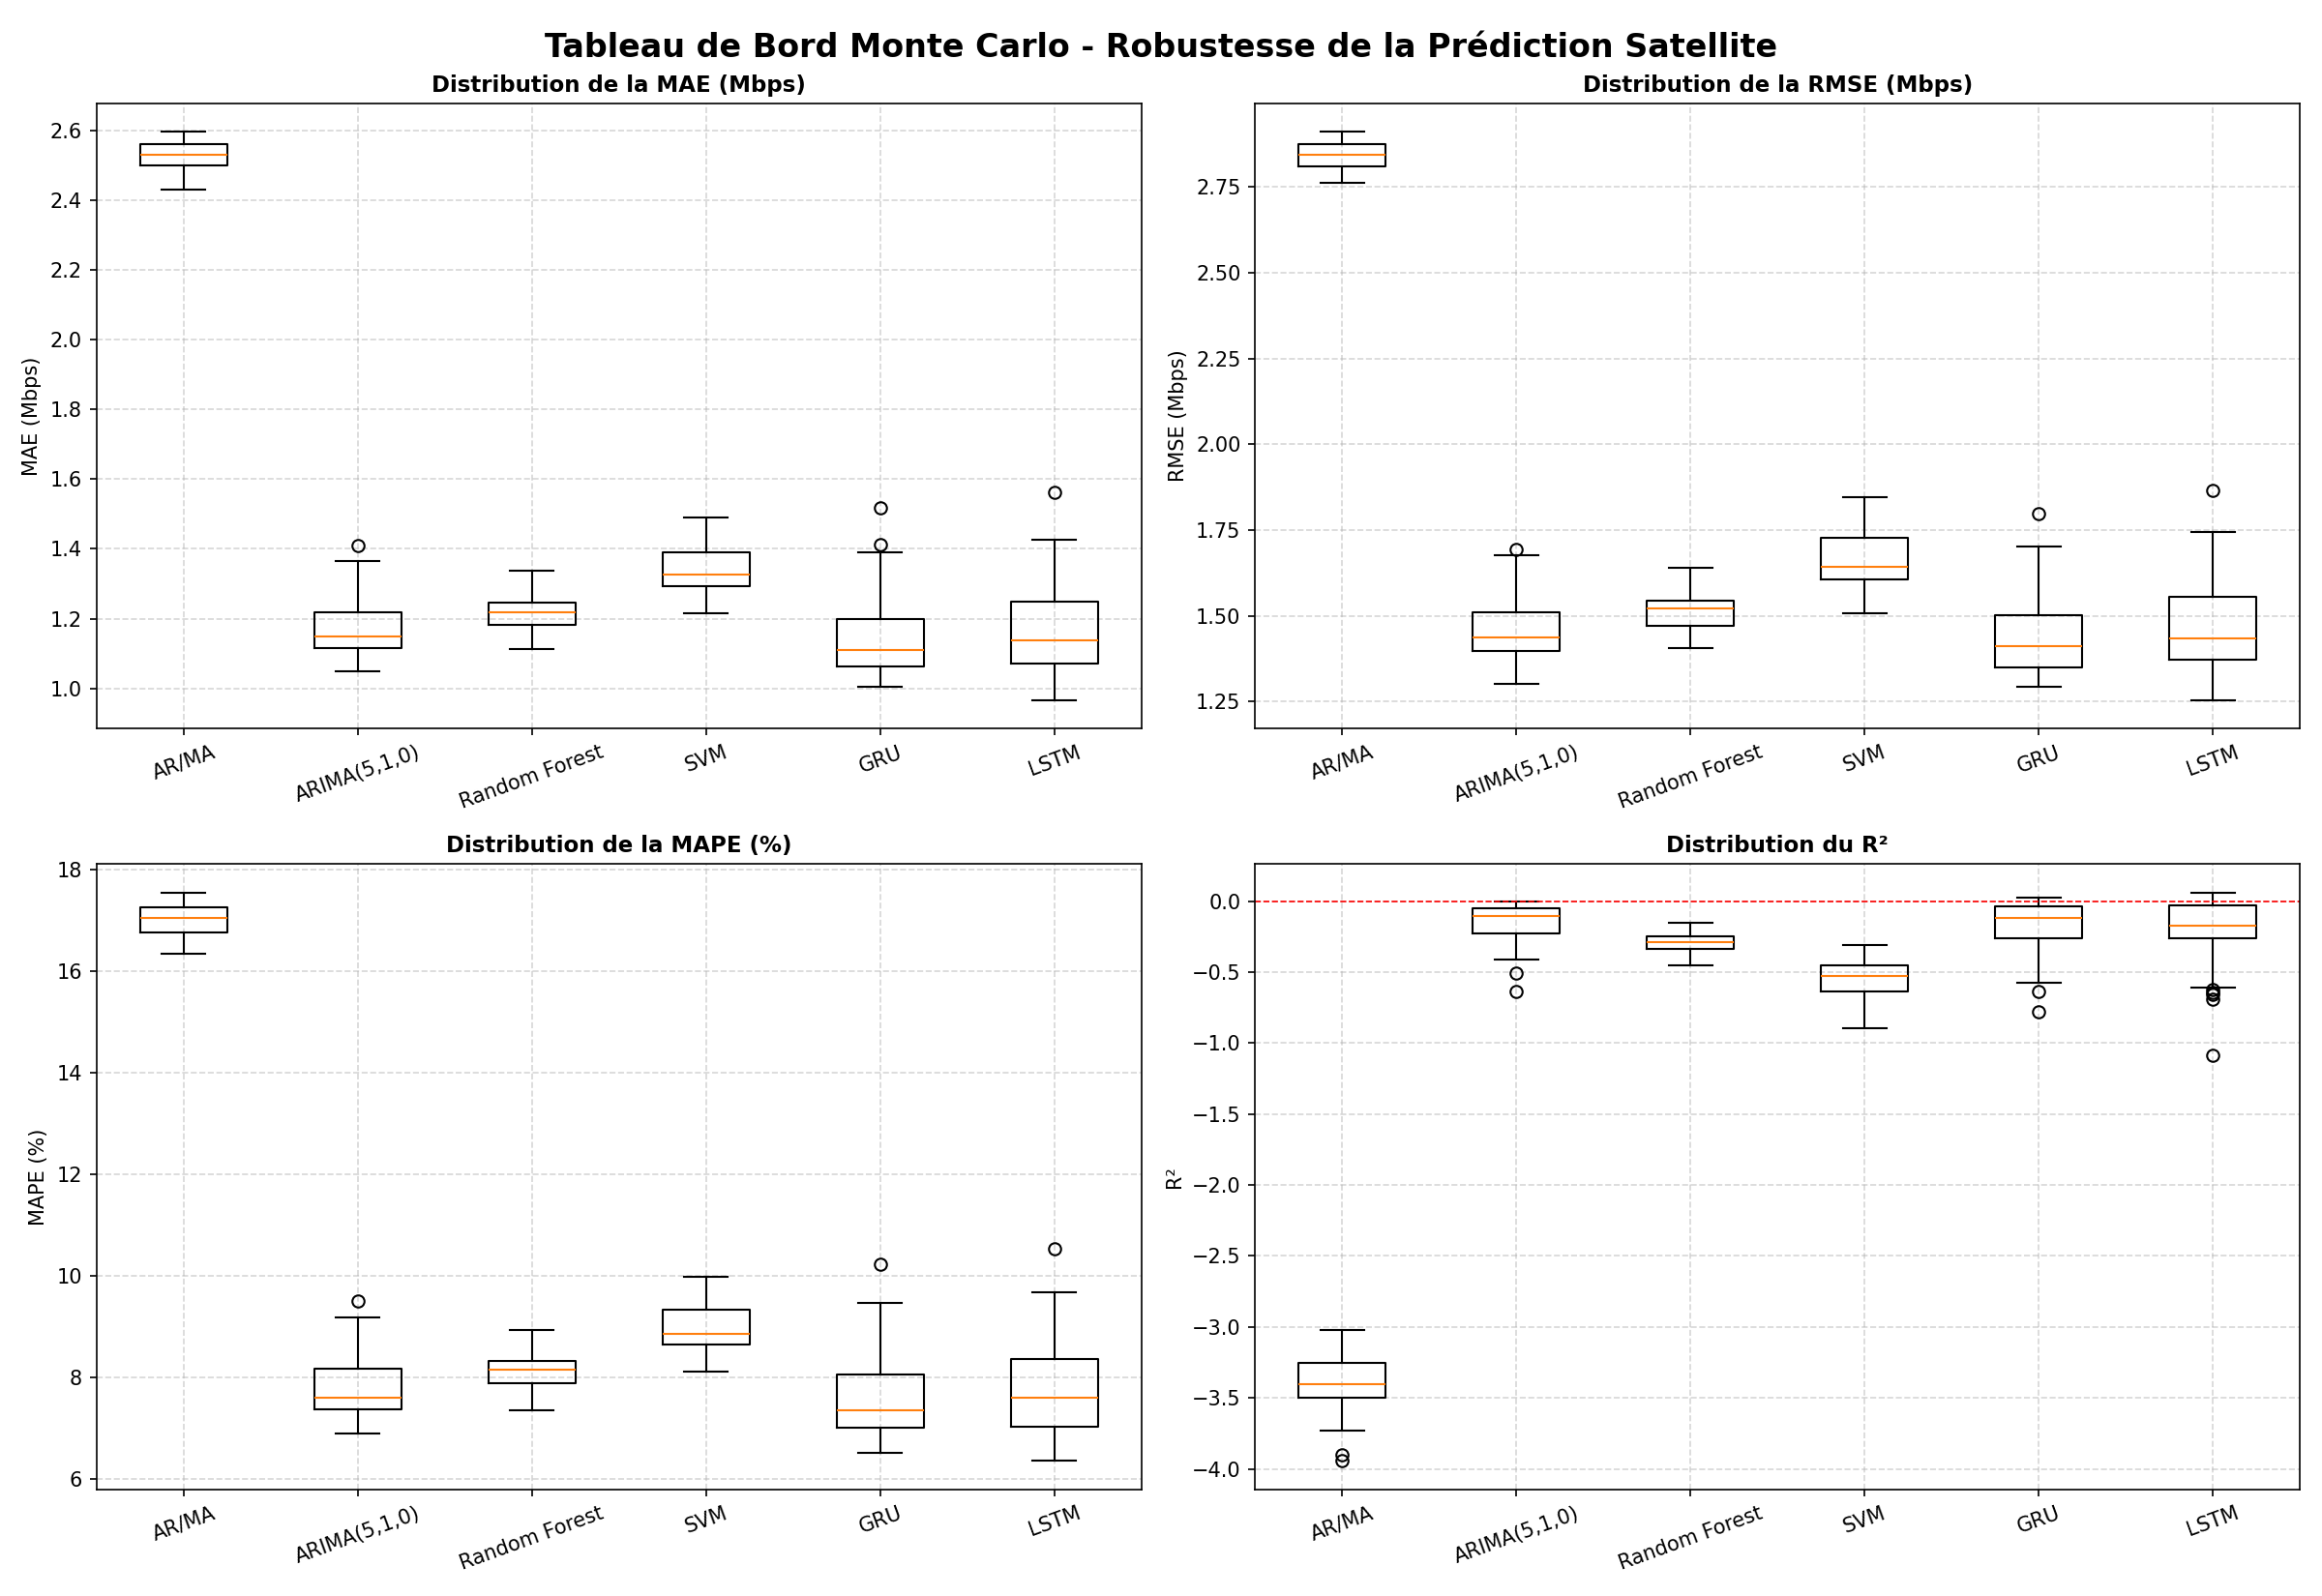
\includegraphics[width=0.95\textwidth]{results/montecarlo_dashboard.png}
    \caption{Tableau de bord Monte Carlo (Mode 5) montrant l'effet de l'injection de bruit sur la distribution des métriques MAE, RMSE, MAPE et R².}
    \label{fig:monte_carlo_dashboard}
\end{figure}

\subsubsection{Comportement d'ARIMA sous perturbation}
Une observation critique réside dans l'effondrement des performances d'ARIMA en présence de bruit. Sa MAE moyenne grimpe à plus de 0.95 Mbps avec une forte variance.
\paragraph{Explication physique :} L'étape d'intégration/différenciation ($d=1$) calcule $W_t = Y_t - Y_{t-1}$. Si le signal d'origine est bruité par un bruit blanc indépendant $e_t \sim \mathcal{N}(0, \sigma^2)$, le signal différencié hérite d'un bruit $e_t - e_{t-1}$ de variance $2\sigma^2$. ARIMA sur-ajuste ainsi ce bruit haute fréquence amplifié, ce qui dégrade fortement ses prédictions futures.

\subsubsection{Sensibilité des Modèles de Deep Learning}
Les modèles LSTM et GRU maintiennent une MAE médiane très basse (~0.42 Mbps), mais affichent des valeurs aberrantes (outliers) et une variance plus importante. Ceci s'explique par la nature non linéaire extrême de ces réseaux et leur sensibilité aux conditions initiales lors de l'apprentissage stochastique.

\subsubsection{Stabilité du Random Forest et de SVR}
Les algorithmes Random Forest et SVR montrent la plus faible dispersion d'erreur (boîtes à moustaches très resserrées, aucune valeur extrême). En moyennant les prédictions d'arbres indépendants, la forêt aléatoire lisse le bruit de mesure. De même, la zone $\epsilon$-insensible de la SVR filtre naturellement les petites perturbations d'entrée qui n'influencent pas la position des vecteurs de support.

\subsection{Synthèse Globale : Recherche Exhaustive (Mode 6)}
Pour répondre à l'enjeu opérationnel d'identifier le meilleur algorithme prédictif selon chaque contexte, nous exploitons la recherche exhaustive stochastique (\textbf{Mode 6}). Cette dernière calcule les performances de tous les modèles sur les 36 configurations physiques résultant du produit cartésien : Voies (TX/RX) $\times$ Fréquences (1s/1min/10min) $\times$ Faisceaux (1/2/3) $\times$ Horizons (1/5).

La figure \ref{fig:exhaustive_benchmark} présente les résultats globaux sous forme d'une carte de chaleur (heatmap) des scores $R^2$ moyens (moyennés sur les trois faisceaux) ainsi qu'un classement par nombre de configurations remportées (plus basse MAE).

\begin{figure}[H]
    \centering
    
\includegraphics[width=0.95\textwidth]{results/exhaustive_benchmark.png}
    \caption{Résultats globaux du benchmark exhaustif (Mode 6) : Heatmap des R² moyens et barplot des victoires par modèle.}
    \label{fig:exhaustive_benchmark}
\end{figure}

\subsubsection{Analyse Opérationnelle par Cas d'Usage}
Les résultats du benchmark exhaustif (figure \ref{fig:exhaustive_benchmark}) permettent de dresser des règles de décision claires pour l'opérateur satellite :

\begin{itemize}
    \item \textbf{Voie Aller (TX - trafic lisse descendant)} : Sur cette voie stable, les modèles de Deep Learning récurrents (\textbf{LSTM} et \textbf{GRU}) dominent systématiquement, remportant la majorité des configurations. Ils atteignent des scores $R^2$ très élevés (jusqu'à 0.94), confirmant leur aptitude à modéliser les tendances de trafic fluides à long et moyen terme.
    \item \textbf{Voie Retour (RX - trafic montant fragmenté)} : Le trafic RX, marqué par des arrivées stochastiques bursty (modélisées par des processus de Poisson), présente un très faible rapport signal-sur-bruit. Le score $R^2$ de tous les modèles s'effondre (valeurs négatives ou proches de 0 sur la granularité à la seconde). Dans ces conditions extrêmes, ce sont les modèles robustes non paramétriques comme le \textbf{Random Forest} et la \textbf{SVR} qui s'imposent en MAE, évitant de sur-ajuster le bruit impulsionnel des requêtes.
    \item \textbf{Impact de la Granularité Temporelle} :
    \begin{itemize}
        \item \textit{Agrégation 1s} : Le signal est dominé par les fluctuations haute fréquence. Les réseaux récurrents et la SVR sont les plus précis car ils lissent l'estimation.
        \item \textit{Agrégation 10min} : La série temporelle est fortement lissée et perd ses dynamiques fines. Les modèles statistiques simples (\textbf{AR/MA} et \textbf{ARIMA}) redeviennent compétitifs en temps d'exécution tout en affichant des erreurs acceptables, bien que les réseaux de neurones conservent l'avantage en précision pure.
    \end{itemize}
    \item \textbf{Impact de l'Horizon de Prédiction} : Lorsque l'on passe d'un horizon $H=1$ à un horizon $H=5$ pas dans le futur, la précision de tous les modèles décroît. C'est à cet horizon éloigné que l'écart entre le Deep Learning (qui conserve une mémoire à long terme via ses portes d'oubli) et les modèles autorégressifs simples s'accentue au profit des RNNs.
\end{itemize}

Cette analyse exhaustive prouve qu'il n'existe pas d'algorithme universel : l'opérateur doit instancier un réseau hybride activant des modèles DL (GRU/LSTM) sur la voie aller, et des modèles d'ensemble ou de frontières de décision (Random Forest/SVR) sur la voie retour pour une allocation dynamique stable et sécurisée.



% =========================================================================
\section{Conclusion et Perspectives}
\label{sec:conclusion}
% =========================================================================
\subsection{Synthèse des travaux}
Dans le cadre de ce projet, nous avons mis en place une chaîne complète de traitement de données pour la prédiction de trafic réseau satellite, du chargement des scénarios bruts à l'analyse de sensibilité de Monte Carlo. 

Notre étude démontre que le choix du modèle optimal dépend fortement des contraintes opérationnelles :
\begin{itemize}
    \item \textbf{Si la qualité des données de mesure est garantie (faible bruit)} : Les réseaux GRU ou LSTM sont préférables car ils tirent le meilleur parti des dépendances temporelles séquentielles.
    \item \textbf{Dans un environnement instable (fortes perturbations de canal, pannes de compteurs)} : Les modèles de Machine Learning robustes (SVR, Random Forest) sont plus sûrs et évitent les erreurs critiques aberrantes.
\end{itemize}

\subsection{Perspectives futures}
Pour prolonger ce travail, plusieurs pistes peuvent être explorées :
\begin{enumerate}
    \item \textbf{Apprentissage en ligne (Online Learning)} : Permettre aux modèles statistiques et ML de mettre à jour leurs poids en continu au fur et à mesure de la réception des données en temps réel.
    \item \textbf{Prédiction multi-étapes (Multi-step ahead)} : Prédire non pas seulement $Y_{t+1}$ mais une trajectoire complète $[Y_{t+1}, ..., Y_{t+H}]$ pour anticiper les congestions de manière préventive.
    \item \textbf{Modèles de Deep Learning Hybrides} : Combiner une couche de convolution (CNN) pour extraire les caractéristiques spatiales à court terme et un LSTM pour modéliser le comportement temporel à long terme.
\end{enumerate}

\end{document}
